\documentclass[../main/main.tex]{subfiles}

\newdate{date}{20}{11}{2019}


\begin{document}

\marginpar{ \textbf{Lecture 11.} \\  \displaydate{date}. \\ Compiled:  \today.}

The partition function is

\begin{equation}
Z_N (T,J,H) = \sum_{\{ S \}  }^{} \exp [\frac{\beta J}{2N} \sum_{ij}^{} S_i S_j + \beta H \sum_{i}^{} S_i    ]
\end{equation}
Since there are no restrictions on the double sum, we can write
\begin{equation*}
  \sum_{ij}^{} S_i S_j  = \qty(\sum_{i}^{} S_i ) \qty(\sum_{j}^{} S_j )= \qty( \sum_{i}^{} S_i )^2
\end{equation*}
Rewriting the partition function, we have:
\begin{equation}
  Z_N (T,J,H)  =   \sum_{\{ S \}  }^{} \exp  [\frac{K}{2N} \qty( \sum_{i}^{} S_i )^2 + h \sum_{i}^{} S_i    ]
\end{equation}
\begin{remark}
Recall that we have defined \(K=\beta J\) and \( h = \beta H\).
\end{remark}

In order to transform the quadratic term into a linear one we make use of the integral identity known as the \emph{Hubbard–Stratonovich transformation} (we can do it in any dimension). 
Let 
\begin{equation*}
 x \equiv \sum_{i}^{} S_i
\end{equation*}
The key identity in the Hubbard-Stratonovich method is simply an observation of the result of a Gaussian
integral. In the present case it takes the form
\begin{empheq}[box=\myyellowbox]{equation}
  e^{\frac{K x^2}{2N}} =  \sqrt{\frac{N K}{2 \pi }} \int_{-\infty }^{+\infty } e^{-\frac{N K}{2}y^2+Kxy} \dd[]{y}, \qquad \Re K >0
  \label{eq:11_1}
\end{empheq}
where \emph{y} is a random field that follows a random distribution.
\begin{proof}[Proof of Hubbard-Stratonovich identity]
To show the identity \eqref{eq:11_1} it is sufficient to complete the square
  \begin{equation*}
    - \frac{N K}{2} y^2 + K x y = - \frac{N K}{2} \qty(y - \frac{x}{N})^2 + \frac{K x^2}{2N}
  \end{equation*}
and then shifting the integral to one over \(z \equiv \qty( y - \frac{x}{N} )\).

Hence,
  \begin{equation*}
    e^{\frac{K x^2}{2N}} \int_{- \infty }^{+ \infty } e^{- \frac{N K}{2} \qty(y - \frac{x}{N})^2 } \dd[]{y} \overset{(a)}{=}  e^{\frac{K x^2}{2N}} \sqrt{\frac{2 \pi }{N K}}
  \end{equation*}
  where in \( (a) \) we have considered \( z \equiv \qty( y - \frac{x}{N} )\) , \( \dd[]{z} = \dd[]{y}   \) and the integral
  \begin{equation*}
    \int_{-\infty }^{+\infty } e^{- \alpha z^2} \dd[]{z} = \sqrt{\frac{\pi }{\alpha }}
  \end{equation*}
  with \( \alpha \equiv \frac{N K}{2} \).
  
\end{proof}
By using \eqref{eq:11_1} in the partition function, we have
\begin{equation}
  Z_N (K,h)= \sqrt{\frac{N K}{2 \pi }} \int_{-\infty }^{+ \infty } \dd[]{y} e^{- \frac{NK}{2}y^2} \underbrace{\qty[\sum_{\{ S \}  }^{}  e^{(h+Ky) \sum_{i}^{} S_i  }  ]}_{Q_y}
\end{equation}
where
\begin{equation}
 Q_y  =  \sum_{\{ S \}  }^{}  e^{(h+Ky) \sum_{i=1}^{N} S_i  }
      = \prod_{i=1}^{N} \qty(\sum_{S_i = \pm 1}^{} \exp [ (h+Ky) S_i]  )
      = \qty( 2 \cosh (h+Ky))^N
\end{equation}
\begin{remark}
\emph{y} is called \emph{auxiliary field} and is a fluctuating external field  with Gaussian distribution.
\end{remark}
The partition function becomes
\begin{equation}
Z_N (K,h) = \sqrt{\frac{N K}{2 \pi }} \int_{- \infty }^{+ \infty } \dd[]{y} e^{- \frac{NK}{2}y^2} \qty(2 \cosh(h+Ky))^N = \sqrt{\frac{N K}{2 \pi }} \int_{-\infty }^{+\infty } \dd[]{y} e^{N \mathcal{L} (K,h,y)}
\end{equation}
where
\begin{equation}
  \mathcal{L} (K,h,y) = \ln{\qty[2 \cosh(h+Ky)] } - \frac{K}{2}y^2
\end{equation}

\begin{remark}
In the limit \( N \rightarrow \infty  \) the integral can be computed exactly by the \emph{saddle point method}.
We can replace the medium of the integral with the maximum of the integrand, we say that all the information is coming only from a bit of information. Replacing the all integral with the integrand computed where it is maximum is an approximation and we are loosing information.  It also depends on the form of the function. For example, for a delta function it works better. In general:
\begin{equation*}
  \int_{-\infty }^{+ \infty } f(x) \dd[]{y} \rightarrow f(\bar{x} )
\end{equation*}
where \( \bar{x} = \max_{x} f(x)  \).
\end{remark}


Indeed as \( N \rightarrow \infty  \), since the integrand is \( \exp (N \mathcal{L} (K,h,y))  \), the integral is dominated by the global maximum in \emph{y} of the function \( \mathcal{L} (K,h,y) \):
\begin{equation*}
  Z_N (K,h) \overset{N \gg1 }{\approx}  \sqrt{\frac{N K}{2 \pi }} \max_y \qty[e ^{N \mathcal{L}(K,h,y) } ]
\end{equation*}
Let \( y_s \) be the value of \( y \) at which
\begin{equation*}
  \mathcal{L} (K,h,y_s) = \max_y \mathcal{L} (K,h,y)
\end{equation*}
hence,
\begin{equation}
  Z_N (K,h) \overset{N \gg1 }{\approx} \sqrt{\frac{N K}{2 \pi }} e^{N \mathcal{L} (K,h,y_s)}
\end{equation}
When we are able to compute the \( y_s \) we can do this approximation and we can compute the bound free energy as 
\begin{equation}
  f_b (K,h)= \lim_{N \rightarrow \infty } \frac{1}{N} \qty(- k_B T \log{Z_N}) = -k_B T \mathcal{L} (K,h,y_s)
\end{equation}


\begin{example}{How to compute \( y_s \)}{}
Looking for \( y_s \), we consider the condition of maximum \( \pdv{\mathcal{L} }{y} = 0  \):
\begin{equation}
  \pdv{\mathcal{L}}{y} = \frac{\sinh (h+Ky)K}{\cosh (h+Ky)} - Ky = 0 \quad   \Rightarrow y_s = \tanh (h+Ky_s)
  \label{eq:11_3}
\end{equation}
The last one is an implicit equation that can be solved graphically as a function of \emph{K} and \emph{h}.
\end{example}

The magnetization in the \( N \rightarrow \infty  \) limit is given by
\begin{equation*}
\begin{split}
m  &= - \qty( \pdv{f}{H})_T = \lim_{N \rightarrow \infty } \frac{1}{\beta N} \pdv{\ln{Z_N(K,h)} }{H}   \\
& =  \pdv{\mathcal{L} (K,h,y_s) }{h}  + \frac{O ( \log{N} )}{N} = \frac{2 \sinh(Ky_s+h)}{2 \cosh(K y_s+h)} \\
& = \tanh (K y_s +h)
\end{split}
\end{equation*}
Hence, showing that \(y_s\) is determined by Eq.\eqref{eq:11_3} plays the role of an effective field acting on each spin. Comparing Eq.\eqref{eq:11_3} with the last result, gives us the self consistency condition for \(m\)
\begin{equation}
   m \equiv y_s \Rightarrow \quad m = \tanh (h+Km)
\end{equation}
\begin{remark}
We have solved analitically this problem.
This is the usual “mean field” result.
\end{remark}
\begin{remark}
The a Hubbard-Stratonovich transformation is generally useful for transforming an interacting problem to a sum or integration over non-interacting problems.
\end{remark}











\chapter{Mean field theories of phase transitions and variational mean field}

\section{Mean field theories}

Increasing the dimension of the systems, the effort to solve analitically the problems increase; indeed, we have seen that
\begin{itemize}
\item In \( d=1 \): many (simple) models can be solved exactly using techniques such as the transfer matrix method.
\item In \( d=2 \): few models can still be solved exactly (often with a lot of effort).
\item In \( d=3 \): almost no model can be exactly solved.
\end{itemize}
Hence, approximations are needed.
The most important and most used one is the \emph{mean field approximation}. 
It has different names depending on the system considered:
\begin{itemize}
\item Magnetic systems: Weiss theory.
\item Fluids systems: Van der Walls.
\item Polymers: Flory's theory.
\end{itemize}

The idea is trying to simplify the problem by neglecting the correlation between the fluctuations of the order parameter. It is equivalent to a statistical independence of the microscopic degrees of freedom.



\subsection{Mean field for the Ising model}
Let us start from the generic Ising model
\begin{equation}
  \mathcal{H} [\{ S \}  ] =  -\frac{1}{2} \sum_{ij}^{} J_{ij} S_i S_j - H \sum_{i}^{} S_i
\end{equation}
where the double sum over \( i \) and \( j \) have no restrictions, while \( H \) is homogeneous.

The partition function is
\begin{equation}
  Z_N (T,H,\{ J_{ij} \}  )= \sum_{\{ S \}  }^{} e^{-\beta   \mathcal{H} [\{ S \}] } = \exp (-\beta F_N (T,H,\{ J_{ij} \}  ))
\end{equation}
Since \( H \) is uniform, the magnetization per spin is
\begin{equation*}
  \expval{S_i}  = \expval{S} \equiv m
\end{equation*}
Let us now consider the identity
\begin{equation*}
\begin{split}
  S_i S_j  &= (S_i - m + m) (S_j - m + m)  \\
  & = (S_i - m ) (S_j - m)  + m^2 + m (S_j-m) + m (S_i-m)
\end{split}
\end{equation*}

\begin{remark}
The mean field approximation consists in neglecting the term
\begin{equation*}
  (S_i - m ) (S_j - m) = (S_i - \expval{S_i})(S_j - \expval{S_j})
\end{equation*}
that measures correlation between fluctuations. 
\end{remark}

Hence, using the mean field approximation, the above identity becomes
\begin{equation*}
  S_i S_j  \approx m^2 + m(S_i-m) + m(S_j-m)
\end{equation*}
and
\begin{equation*}
  \frac{1}{2} \sum_{i,j}^{} J_{ij}S_i S_j \overset{MF}{\approx } \frac{1}{2} \sum_{i,j }^{} J_{ij} \qty[-m^2+m(S_i+S_j)]
\end{equation*}
Let us focus on the term
\begin{equation}
  \frac{1}{2} \sum_{i,j }^{} J_{ij} m (S_i+S_j) = 2 \frac{1}{2} m \sum_{i,j }^{} J_{ij}  S_i
  \label{eq:11_2}
\end{equation}
If we do not make any assumption on \( J_{ij} \), the mean field Hamiltonian is
\begin{equation}
\mathcal{H}_{MF} [ \{ S \}  ] = \frac{1}{2} m^2 \sum_{ij}^{} J_{ij} - m \sum_{ij}^{} J_{ij} S_i - H \sum_{i}^{} S_i
\end{equation}
and by calling
\begin{equation*}
  \bar{J_i} \equiv  \sum_{j}^{} J_{ij}
\end{equation*}
we get
\begin{equation*}
    \mathcal{H}_{MF} [ \{ S \}  ]  = \frac{1}{2} m^2 \sum_{i}^{} \bar{J_i} - \mathcolorbox{green!20}{\frac{m}{2}} \sum_{i}^{} \bar{J_i} S_i - H \sum_{i}^{} S_i
\end{equation*}
\begin{remark}
Note the coefficient emphasized in green (\( 1/2 \)) is needed to avoid the double counting of bonds.
\end{remark}
Moreover, if we suppose that
\begin{equation*}
  \bar{J_i} \rightarrow \bar{J}
\end{equation*}
we have
\begin{empheq}[box=\myyellowbox]{equation}
  \mathcal{H}_{MF} [ \{ S \}  ] = \frac{1}{2} m^2 N \bar{J} - \qty(\frac{m}{2}\bar{J} +H) \sum_{i}^{} S_i
\end{empheq}
\begin{remark}
In the standard Ising model, where
\begin{equation*}
  \frac{1}{2} \sum_{ij}^{} J_{ij} S_i S_j \rightarrow \sum_{\expval{ij} }^{} J_{ij}    S_i S_j
\end{equation*}
the term \( 2 m \sum_{\expval{ij} }^{}  J_{ij} S_i \) of Eq.\eqref{eq:11_2} can be written as follows.
Let
\begin{equation*}
  \sum_{j \in n.n.\text{ of } i}^{} J_{ij} = z \hat{J}_i
\end{equation*}
where \( z \) is the coordination number of the underlying lattice (for the hypercubic lattice \( z=2d \)).
By assuming \( \hat{J}_i = \hat{J}  \) and inserting the \( 1/2 \) to avoid double counting, we have that equation \eqref{eq:11_2} becomes
\begin{equation}
  2m \sum_{\expval{ij} }^{}  J_{ij} S_i = 2 m \frac{1}{2} z \hat{J} \sum_{i=1}^{N} S_i
\end{equation}
\end{remark}

Hence, in this case the Hamiltonian is
\begin{empheq}[box=\myyellowbox]{equation}
  \mathcal{H}_{MF} [ \{ S \}  ] = \frac{1}{2} m^2 N z \hat{J} - (m z \hat{J} + H ) \sum_{i=1}^{N} S_i
\end{empheq}
The partition function becomes
\begin{equation}
\begin{split}
  Z_N (T,H,\hat{J} ) &= e^{-N \beta \hat{J} \frac{z}{2} m^2 }  \sum_{\{ S \}  }^{} e^{\beta  (\hat{J}zm+H )\sum_{i=1}^{N} S_i }   \\
  & = e^{-N \beta \hat{J} \frac{z}{2} m^2 } \prod_{i=1}^{N}  \sum_{S = \pm 1}^{} \exp (\beta  \qty(\hat{J}zm+H ) S_i )   \\
  & = e^{-N \beta \hat{J} \frac{z}{2} m^2 } \qty(2 \cosh \qty[\beta \qty(\hat{J}zm+H ) ] )^N
\end{split}
\end{equation}
\begin{remark}
We are replacing the interaction of the J with a field close to the \( S_i \). We called \( \hat{J} z m = H_{eff}  \), the mean field!
\end{remark}

The free energy per spin is
\begin{equation}
\begin{split}
  \frac{F_N (T,H,\hat{J} )}{N} & = \frac{1}{N} \qty(-k_B T \ln{Z_N(T,H,\hat{J} )} ) \\
  & = \frac{1}{2} \hat{J} z m^2 - k_B T \ln{\qty[\cosh(\beta (\hat{J}zm+H ))] } - k_B T \ln{2}
\end{split}
\end{equation}
Sometimes it is useful to use the \emph{dimensionless variables} defined as
\begin{equation}
  \bar{f} \equiv \frac{F_N}{N z \hat{J} }, \quad \theta \equiv \frac{k_B T}{z \hat{J} }, \quad \bar{H} \equiv \frac{H}{z \hat{J} }
\end{equation}
Hence,
\begin{equation}
  \bar{f} (m, \bar{H}, \theta  ) = \frac{1}{2}m^2 - \theta \ln{\qty(2 \cosh (\theta ^{-1}(m+\bar{H} ))) }
\end{equation}

In order to be a self-consistent, the last equation has to satisfy the  thermodynamic relation:
\begin{equation*}
  m = - \qty( \pdv{f}{H})_T \quad \Rightarrow   m = \tanh (\beta (\hat{J}z m + H  ))
\end{equation*}
\begin{remark}
The results of \( m \)  is similar to the Ising with infinite range (\( \hat{J}z \leftrightarrow J  \)).
\end{remark}

Now, let us consider the \( H=0 \) case, we have
\begin{equation}
  m =  \tanh (\beta (\hat{J}z m ))
\end{equation}
and the graphical solution is shown in Figure \ref{fig:11_1} (hyperbolic function).
We can distinguish three cases:
\begin{itemize}
\item Case \( \beta \hat{J} z > 1  \): there are three solutions, one at \( m=0 \) and two symmetric at \( m=\pm m_0 \). Magnetization is \( \neq 0 \, (= \abs{m_0} )\) for \( H=0 \) (\emph{ordered phase}).  The two solution are symmetric because they are related by the \( \mathbb{Z}^2 \)  symmetry.
\item Case \( \beta \hat{J} z < 1  \): single solution at \( m=0 \) (\emph{disordered or paramagnetic phase}).
\item Case \( \beta \hat{J} z = 1  \): the three solutions coincide at \( m=0 \) (\emph{critical point}). 
The critical temperature \( T_c \) is given by
\begin{equation*}
 \beta_c \hat{J} z = 1 \Rightarrow  \frac{z \hat{J} }{k_B T_c} = 1 \Rightarrow T_c = \frac{z \hat{J} }{k_B} \neq 0!
\end{equation*}
\begin{remark}
\( T_c \) depends on \emph{z} and hence on \emph{d}!
\end{remark}
\end{itemize}



\begin{figure}[h!]
\centering
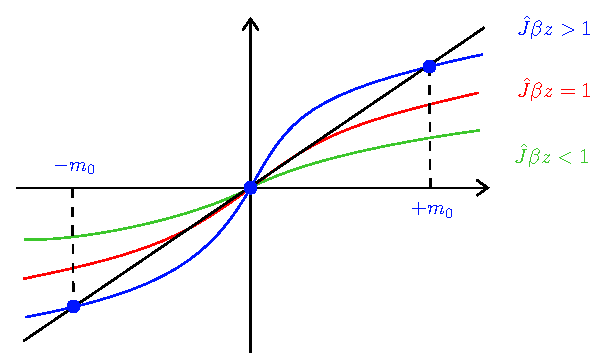
\includegraphics[width=0.9\textwidth]{../lessons/11_image/1.pdf}
\caption{\label{fig:11_1} Graphical solution of equation \(m =  \tanh (\beta (\hat{J}z m )) \) (case \(H=0\)).}
\end{figure}


\subsection{Free-energy expansion for \( \pmb{m \simeq 0} \) }
The critical point is characterized by the order parameter that is zero. Now, we want to expand the free energy around the critical point. Let us put \( H=0 \):
\begin{equation}
  f(m,0,T,\hat{J} ) = \frac{1}{2}\hat{J}zm^2 -k_BT \ln{\qty[\cosh(\beta \hat{J}zm )]}
\end{equation}
Define \( x \equiv \beta \hat{J} z m \simeq 0  \) and by expanding in Taylor series
\begin{equation*}
  \cosh (x) \simeq 1 + \underbrace{\frac{x^2}{2} + \frac{x^4}{4!}}_{t \simeq 0}  + \dots
\end{equation*}
\begin{equation*}
  \log{(1+t)} \simeq t - \frac{1}{2}t^2
\end{equation*}
Hence,
\begin{equation*}
  \log{(\cosh x)} \simeq \frac{x^2}{2} + \frac{x^4}{4!} - \frac{1}{2} \frac{x^4}{4}+O(x^6)
  = \frac{x^2}{2} - \frac{x^4}{12}+O(x^6)
\end{equation*}
This gives the result
\begin{equation}
  f(m,0,T,\hat{J} ) \simeq  const + \frac{A}{2} m^2 + \frac{B}{4} m^4 + O (m^6)
\end{equation}
with
\begin{subequations}
\begin{align}
   A & \equiv  \hat{J} z \qty(1- \beta \hat{J} z) \\
    B & \equiv  \beta ^2 \frac{(\hat{J}z )^4}{3} > 0
\end{align}
\end{subequations}

We have three cases:

\begin{itemize}
\item Case \( \beta \hat{J} z > 1 \Rightarrow A<0 \): two stable symmetric minima at \( m= \pm m_0 \) (Figure \ref{fig:11_2}). Coexistence between the two ordered phases.
\begin{figure}[h!]
\centering
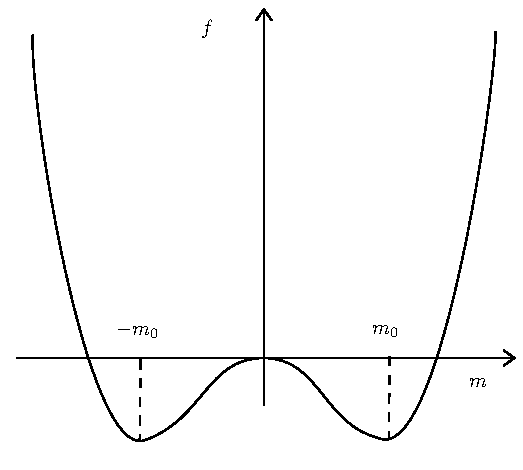
\includegraphics[width=0.4\textwidth]{../lessons/11_image/2.pdf}
\caption{\label{fig:11_2} Plot of the free energy: case \( \beta \hat{J} z > 1 \Rightarrow A<0 \).}
\end{figure}

\item Case \( \beta \hat{J} z < 1 \Rightarrow A>0 \): one minimum at \( m=0 \) (Figure \ref{fig:11_3}).
\begin{figure}[h!]
\centering
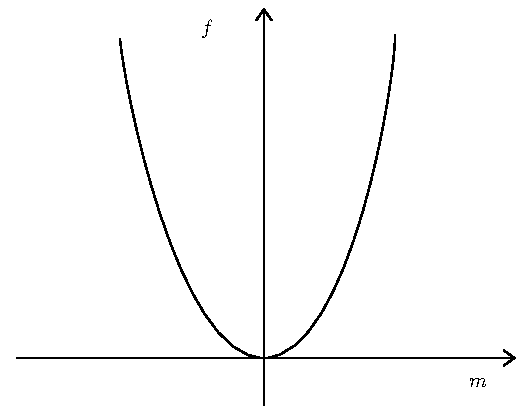
\includegraphics[width=0.4\textwidth]{../lessons/11_image/3.pdf}
\caption{\label{fig:11_3} Plot of the free energy: case \( \beta \hat{J} z < 1 \Rightarrow A>0 \).}
\end{figure}

\item Case \( \beta \hat{J} z = 1 \Rightarrow A=0 \): 3 minima coincide at \( m=0 \) (Figure \ref{fig:11_4}).
\begin{figure}[h!]
\centering
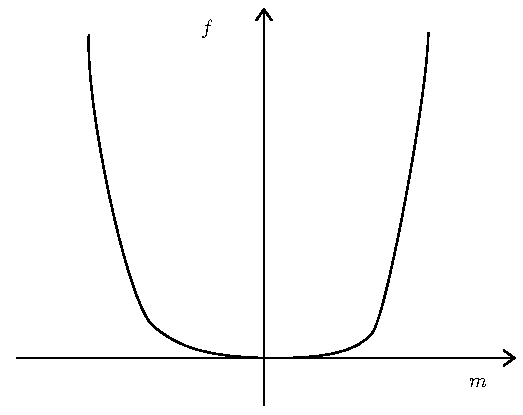
\includegraphics[width=0.4\textwidth]{../lessons/11_image/4.pdf}
\caption{\label{fig:11_4} Plot of the free energy: case \( \beta \hat{J} z = 1 \Rightarrow A=0 \).}
\end{figure}
\end{itemize}




\end{document}
